\chapter{Implémentation}

\section{Implémentation des différents éléments}

La maquette finale de la graveuse laser intelligente est constituée de plusieurs éléments matériels et logiciels qui interagissent pour assurer son bon fonctionnement. Ces éléments principaux sont :

\begin{itemize}
    \item \textbf{Bras robot Ufactory Xarm6}
    \item \textbf{Graveuse laser Creality Falcon}
    \item \textbf{Écran tactile ED-HMI3010-101C}
    \item \textbf{Caméra Intel D435}
\end{itemize}

\section{Bras robot Ufactory Xarm6}

Le bras robot Ufactory Xarm6 est un bras robotique collaboratif à 6 degrés de liberté, offrant une bonne précision et une flexibilité importante pour la manipulation dans l’espace de travail. Le contrôle du bras est réalisé principalement par l’interface graphique AICA Studio qui permet la programmation par blocs fonctionnels.

\subsection{Programmation du bras robot}
La programmation via AICA studio permet un contrôle fin de la cinématique, notamment la gestion des accélérations, vitesses, et positions intermédiaires. Le logiciel offre plusieurs possibilités de contrôle. La communication avec le bras s’effectue par Ethernet.

\subsection{Modifications du bras robot}
La pince fournie par Ufactory à une grande course d'ouverture mais les doigts n'étaient pas très adaptés à la prise de pièces et au placement sous la graveuse laser. Il a donc été nécessaire de concevoir des doigts adaptés à l'utilisation demandée.
\begin{figure}[H]
    \centering
    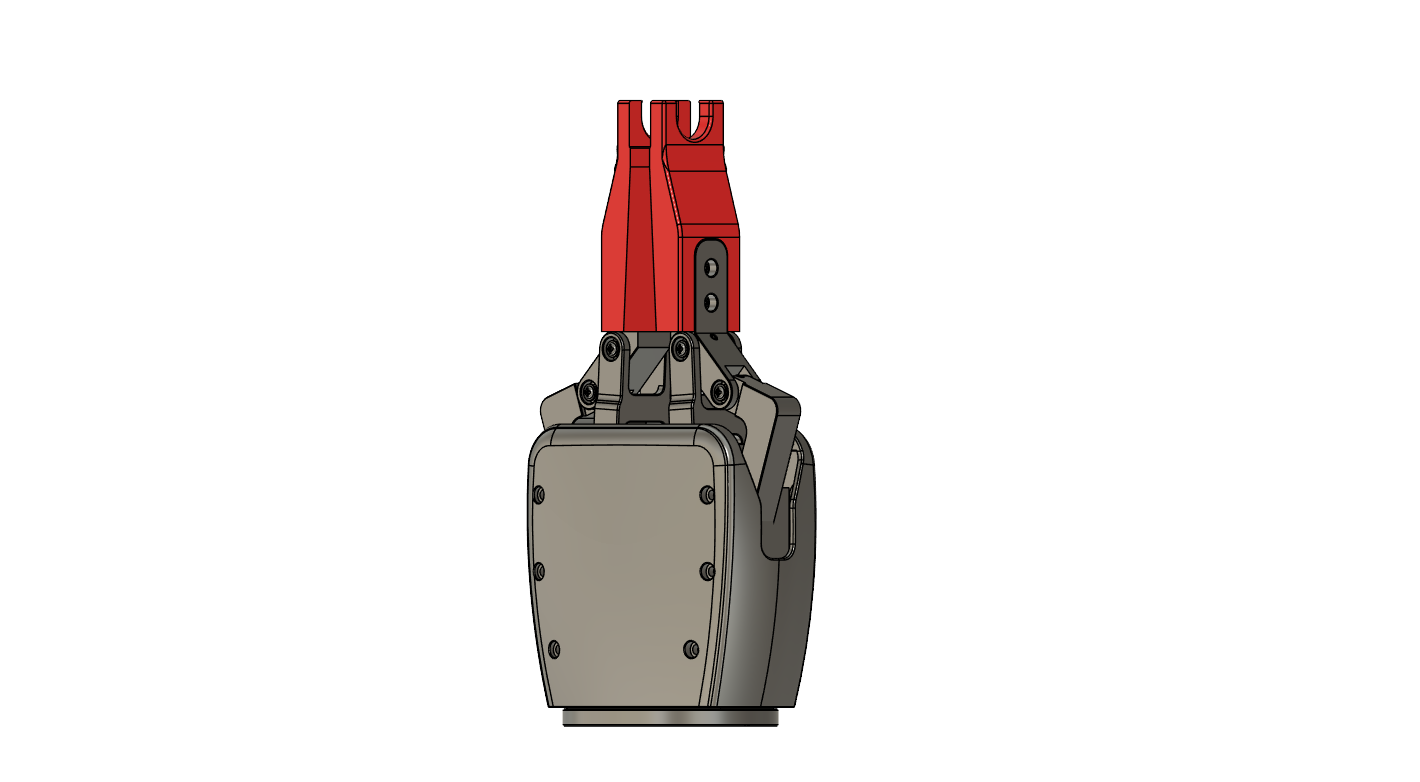
\includegraphics[width=0.8\textwidth]{assets/figures/Pince_Xarm6.png}
    \caption{Pince du bras robot Ufactory Xarm6 modifiée pour la prise de pièces}
    \label{fig:pince_robot}
\end{figure}

\section{Graveuse laser Creality Falcon}

La graveuse laser Creality Falcon est commandée via des fichiers G-code, un langage standard dans le domaine des machines-outils à commande numérique. Les motifs à graver, initialement créés au format \gls{dxf}, sont convertis en fichiers G-code via un script développé spécialement dans le cadre de ce projet.

Ce script réalise les étapes suivantes :
\begin{itemize}
    \item Lecture et analyse des contours du fichier DXF.
    \item Génération de trajectoires compatibles avec le protocole G-code.
    \item Communication entre le logiciel et la graveuse laser.
\end{itemize}

Le fichier G-code généré est ensuite envoyé à la Creality Falcon qui réalise la gravure. Une synchronisation précise avec le bras robot est nécessaire pour assurer que le laser ne s’active que lorsque le bras est en position correcte.

\section{Écran tactile ED-HMI3010-101C}

L’écran tactile ED-HMI3010-101C (appelé ED-101) permet de choisir ce que la graveuse va dessiner. Via une interface graphique, il est possible de dessiner à la main, avec des formes prédéfinies ou avec du texte dans la zone de gravure.

Cette interface est spécialement conçue pour une utilisation en tant que démonstrateur devant du public.

\section{Caméra Intel D435}

La caméra Intel D435 est utilisée pour la détection en 3D des pièces à graver dans l’espace de travail. Grâce à sa capacité à fournir des données de profondeur en temps réel, elle permet :
\begin{itemize}
    \item De localiser précisément les pièces posées sur la zone de travail.
    \item D’adapter la trajectoire du bras robot en fonction de la position exacte des pièces détectées.
\end{itemize}

L’intégration de la caméra dans le système est réalisée via un bloc fonctionnel personnalisé développé dans AICA Studio, utilisant les données 3D captées pour prendre des décisions en temps réel. Le fonctionnement détaillé de ce bloc sera présenté dans le \textbf{chapitre \ref{chap:programmation}}.

\section{Modèle 3D de la maquette}

Le modèle 3D de la maquette a été réalisé à l'aide du logiciel de modélisation 3D Fusion 360. Il permet de visualiser l'ensemble du système, y compris le bras robot, la graveuse laser, l'écran tactile et la caméra. Ce modèle est utilisé dans AICA Studio pour la visualisation de l'espace de travail.

\begin{figure}[H]
    \centering
    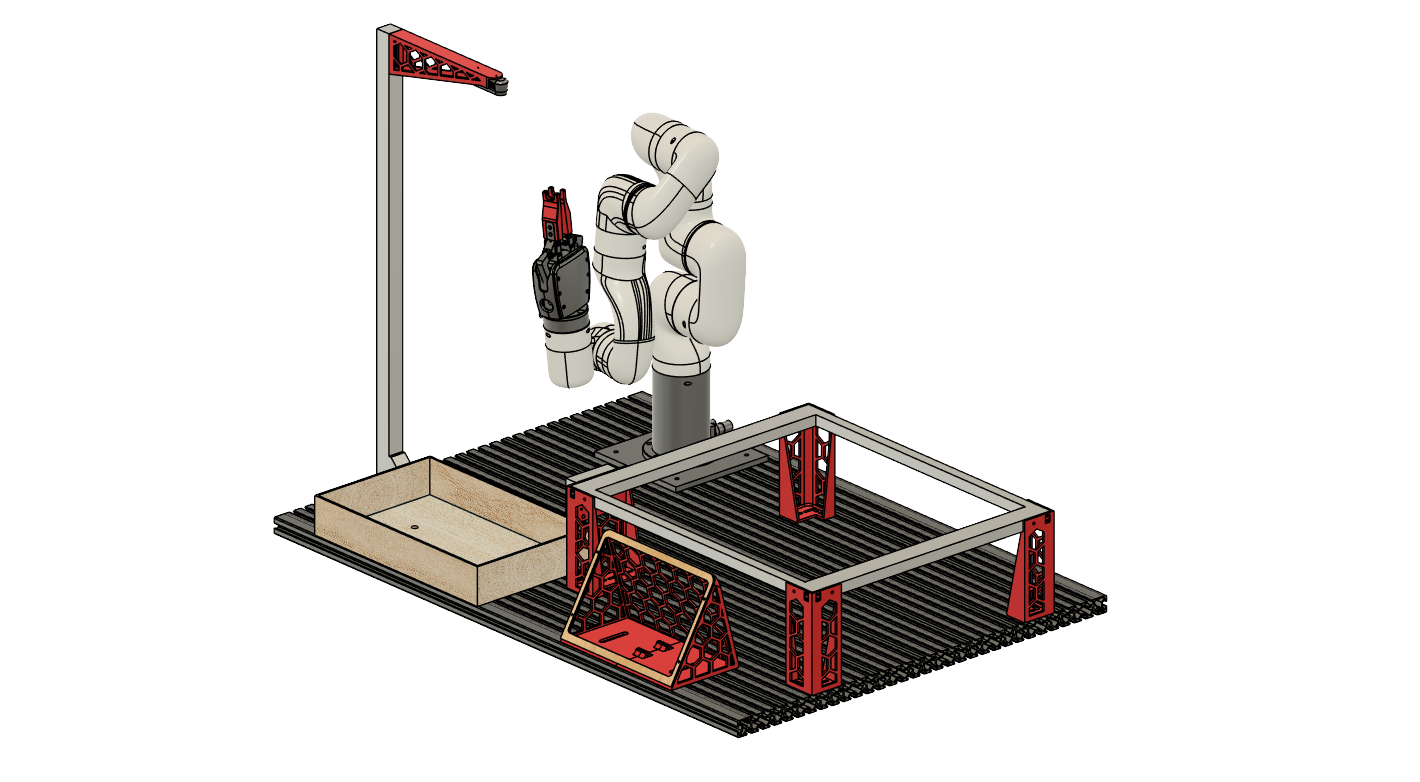
\includegraphics[width=0.8\textwidth]{assets/figures/modele_3d.png}
    \caption{Modèle 3D de la maquette de la graveuse laser intelligente}
    \label{fig:maquette_3d}
\end{figure}

Ce travail de modélisation a été réalisé pour faciliter la conception de pièces mécaniques, et la définition des points de passage du bras robot. Cela évite des erreurs de mesures et permet de mieux visualiser l'ensemble du système avant la fabrication des pièces ainsi que l'encombrement de la maquette.
